\section{Algorithms}
\label{s:algorithms}

\paragraph{}Convex Optimization is a sub field of Optimization which can produce reliable solutions
and can be solved exactly. Many signal processing problems can be formulated as convex 
optimization problems of form
\begin{equation}
 minimize_{x \in R^N} \hspace{4mm}f_1(x) +f_2(x) + ... + f_{n-1}(x) +f_n(x)
\label{3.1}
\end{equation}

\paragraph{}where $f_1, f_2, ..., f_n$ are convex functions defined from $f:R^N$ $\rightarrow$ $R$ where some of the 
functions are non-differentiable, this which rules out our conventional smooth optimization
techniques like Steepest decent method, conjugate gradient method etc. We have explored
the class of algorithms which can solve equation (\ref{3.1}). These methods proceed by splitting, 
in that the functions $f_1, . . . , f_n$ are used individually so as to yield an easily
implementable algorithm. They are called proximal because each non smooth function in \ref{3.1} 
is involved via its proximity operator. Iterative thresholding, projected Landweber, projected
gradient, alternating projections, alternating-direction method of multipliers, alternating
split Bregman are special instances of proximal algorithms. Details of proximal methods are discussed in \cite{Com07}.

\subsubsection{Notations}
\paragraph{}Here after, $R^N$ is the $N$-dimensional euclidean space and domain of function 
$f: R^N  \rightarrow ]-\infty,+\infty]$. \\
\paragraph{}Let $C$ be the non-empty convex subset of $R^N$. The indicator function of $C$ is defined as

\begin{equation}
i_C : x \mapsto \left\lbrace \begin{array}{ll}
0        &  \mbox{if } x \in C\\
+ \infty & \mbox{if } x \notin C 
\end{array} \right.
\label{3.2}
\end{equation}

$p$-norm is defined as ( $\parallel . \parallel_{p}$ )
\begin{equation}
\parallel x \parallel_p = ( |x|^p + |x|^p + |x|^p +... |x|^p )^{\frac{1}{p}}
\label{3.3}
\end{equation}

\paragraph{}The distance form $x \in R^N$ to $C$ is defined as 
\begin{equation}
 D_C(x) =  min_{y \in C} \parallel x - y \parallel
\label{3.4}
\end{equation}

\paragraph{}If $C$ is closed and convex, the projection of $x \in R^N$ onto $C$ is the unique point $P_Cx \in C$
such that $D_C(x) = \parallel x - P_Cx \parallel_2$.

\paragraph{}Sub differential of $f$ is given by
\begin{equation}
 \partial f : R^N \rightarrow 2^{R^N} : x \mapsto { u \in R^N | (\forall y \in R^N) (y-x)^Tu+f(x) \leq f(y))}
\label{3.5}
\end{equation}

\subsection{Proximal Gradient methods}
\label{s:algorithms_pgm}
\paragraph{}One of the widely used convex optimization algorithm is POCS
( Projection Onto Convex Sets ).This algorithm is employed to recover/synthesize a signal
satisfying simultaneously several convex constraints. Let $f_i$ be the indicator function of non-empty
closed convex set $C_i$ modeling a constraint. This reduces to convex feasibility problem, which 
which require us to find a solution such that it lies in the intersection of all convex sets $C_i$. In POCS 
method each set $C_i$ is incorporated by its projection operator $P_{C_i}$. So in each iteration 
$x$ is updated as
\begin{equation}
x_{k+1} = P_{C_1}  P_{C_2} ... P_{C_n}x_k
\label{3.6}
\end{equation}
\paragraph{}However beyond such problems Projection operators are not appropriate and more general operators 
are required to tackle them. Among the various generalizations of the notion of a convex projection 
operator that exist, proximity operators are best suited for our purposes.

\paragraph{}Proximity operators of function $f$ at $x$ is defined as
\newtheorem*{mydef}{Definition}
\begin{mydef}
For every $x \in R^N$, the minimization problem, 

\begin{equation}
 minimize_{y \in C} \hspace{3mm} f(y) + \frac{1}{2} \parallel x-y \parallel_2^2
\label{3.7}
\end{equation}

admits a unique solution which is denoted by $prox_f(x)$.
\begin{equation}
 prox_f(x) :R^N \rightarrow R^N
\label{3.8}
\end{equation}

\end{mydef}

The proximity operator of $f$ is characterized by inclusion 
\begin{equation}
 (\forall(x,p) \in R^N \times R^N) \hspace{3mm} p=prox_f(x) \Leftrightarrow x-p \in \partial f(p) 
\label{3.9}
\end{equation}
If $f$ is differentiable then above equation reduces to 
\begin{equation}
 (\forall(x,p) \in R^N \times R^N) \hspace{3mm} p=prox_f(x) \Leftrightarrow x-p \in \triangledown f(p)
  \label{3.10}
\end{equation}

% Proximity operators have well defined property which make them well suited for 
% Iterative Minimization algorithms. Some of the property of $prox_fx$ operators are
% $prox_fx$ operator is firmly non-expansive i.e.
% \begin{equation}
% \forall x \in R^N \hspace{3mm} \forall y \in R^N 
%   \parallel prox_fx - prox_fy \parallel^2_2 + \parallel (x-prox_fx)-(y-prox_fy)\parallel_2^2 \leq \parallel x-y \parallel_2^2
% \end{equation}
% for more properties refer appendix.Proximity operators are just the extension of how the projection operators
% are used while solving Convex feasibility problem in POCS. 


\paragraph{}We are interested in algorithms which can solve equation (\ref{1.6}) where $n=2$ in reference with
equation (\ref{3.1}). For notational convenience we use $f(x)$ in place of $f_1(x)$ and $\lambda g(x)$ in place of 
$f_2(x)$. Hence our optimization problem is 
\begin{equation}
 minimize_{x \in R^N} \hspace{3mm} f(x) + g(x)
 \label{3.11}
\end{equation}
collectively we say $F(x) = f(x)+g(x)$ where $f(x) =  \parallel Ax-b \parallel_{2}^2$ and $g(x)=\lambda\parallel x \parallel_{1}$

\subsection{Derivation of Soft Thresholding}
\label{s:algorithms_dst}
\paragraph{}In our problem $g(x)=\lambda \parallel x \parallel_{1}$ and $prox_g(x)$ is called soft shrinkage 
thresholding\footnote{Derived by Prof.~Mihir~Arjunwadkar} operator which minimizes following equation.

\begin{equation}
\begin{array}{rl}
prox_gx =& argmin_y \frac{1}{2} \parallel x-y \parallel_{\ell_2}^2 + \lambda \parallel y \parallel_{\ell_1}  
\end{array}
\label{3.12}
\end{equation}

Using definition of the $\ell_1$-norm and the $\ell_2$-norm we have
\begin{equation}
\begin{array}{rl}
prox_gx =& argmin_y \frac{1}{2} \displaystyle\sum\limits_{i=1}^{i=n}(x_i-y_i)^2 + \lambda \displaystyle\sum\limits_{i=1}^{i=n}|y_i|
\end{array}
\label{3.13}
\end{equation}

To find the minimizer in the above minimization problem, we have to consider three case when $y_i>0$, $y_i<0$, $y_i=0$.\\\\

\emph{Case 1 : $y_i > 0$}\\\\

To get the gradient of objective function in equation () we have to differentiate it with respect to each component and 
then equating each components to zero, the $i_{th}$ component is given by

\begin{equation}
 \begin{array}{rl}
  y_i =& x_i -\lambda
 \end{array}
\label{3.14}
\end{equation}

\emph{Case 2 : $y_i < 0$}\\\\

Similarly, considering each component $y_i$ < 0, the minimizer will be given as

\begin{equation}
 \begin{array}{rl}
  y_i =& x_i +\lambda
 \end{array}
\label{3.15}
\end{equation}
  
\emph{Case 3 : $y_i = 0$}\\\\
We have to find the condition for $y_i=0$ to be the unique minimizer. Then for 
\begin{center}
 
$
\begin{array}{ll}
\Rightarrow \frac{1}{2}(x_i^2-2x_iy_i+y_i^2) + \lambda |y_i| > \frac{1}{2}x_i^2\\
\Rightarrow y_i+\frac{1}{2}y_i^2 + \lambda |y_i| > 0\\
\Rightarrow \left\lbrace \begin{array}{ll}
 y_i+\frac{1}{2}y_i^2 + \lambda y_i > 0 & \mbox{ for } y_i>0\\
y_i+\frac{1}{2}y_i^2 - \lambda y_i > 0 & \mbox{ for } y_i<0\\
\end{array}\right.
\end{array}
$
\end{center}
The above inequalities will hold anyways for sufficiently large $y_i$. Let us therefore 
consider $|y_i|$ to be arbitrarily close to zero. If the inequalities above are to hold for
any arbitrarily small $|x_i|$, we must have

\begin{equation}
|x_i|\leq \lambda \mbox{ for } y_i = 0
\label{3.16}
\end{equation}

\paragraph{}Combining equation (\ref{3.14}) and (\ref{3.15}) we get
\begin{equation}
 prox_gx = (|x_i|-\lambda) \times sgn(y_i) \mbox{ if } |y_i| >0
\label{3.17}
\end{equation}
where,

\begin{equation}
sgn(y_i) =\left\lbrace
\begin{array}{ll}
  1 & \mbox{if }y_i>0 \\
  0 & \mbox{if }y_i=0 \\
 -1 & \mbox{if }y_i<0 
\end{array} \right.
\label{3.18}
\end{equation}


Further, incorporating equation (\ref{3.16}), we have soft thresholding operator as 
\begin{equation}
 prox_g(x_i) = max(|x_i|-\lambda) \times sgn(y_i)
\label{3.19}
\end{equation}
Note in above equation $prox$ operator is applied on each of the component of $x$.

\subsection{ISTA and FISTA Algorithms}
\label{s:algorithms_ista}

The ISTA (Iterative Shrinkage-Thresholding Algorithm)and FISTA (Fast Iterative Shrinkage-Thresholding Algorithm) 
\cite{fista} methods minimizes functions of the form
 \begin{equation}
  F({x}) = f({x}) + g({x})
 \end{equation}
 where
 \begin{itemize}
  \item
   $x \in R^N$;
  \item
   $f : R^N \rightarrow R$ : smooth, convex continuously differentiable with Lipschitz continuous gradient $L(f)$:
   $$
    \norm{\grad{f}{x} - \grad{f}{y}}_2 \le L(f) \norm{x - y}_2
    \mbox{ for every } {x}, {y} \in R^N
   $$
   where
   $L(f) > 0$ is the Lipschitz constant for $\grad{f}{x}$; and

  \item
   $g : R^N \rightarrow R$ : continuous, convex, but possibly non-smooth function.
 \end{itemize}

\paragraph{}In each iteration, these algorithms calculate 
\begin{equation}
 x_i = prox_g(x_{i-1}-t_i\triangledown f(x))
\label{3.20}
\end{equation}

where, $t_i$ is the step-size parameter. From definition of proximity operator, when $g(x)=0$
then above equation (\ref{3.20}) is given as
\begin{equation}
 x_i = x_{i-1}-t_i\triangledown f(x)
\label{3.21}
\end{equation}
for minimizing the function with a Lipschitz continuous gradient $L(f)$. On the other hand if
$f(x)=0$, then equation (\ref{3.20}) reduces to 
\begin{equation}
 x_i = prox_g(x_{i-1})
\end{equation}
for minimizing non-differentiable function. Such schemes are called as \emph{forward-backward proximal splitting} (\cite{Com07}).
with forward scheme as gradient step using $f(x)$ and backward or implicit scheme using the function $g(x)$. Further 
$prox$ operator for FISTA and ISTA is soft thresholding operator derived in section 3.3. There are two variants 
of each of these algorithms --- One with a fixed step size $t$ and the other with varying step size $t_i$ or backtracking.
The pseudo codes of these algorithms are discussed in next section.

\subsection{Pseudo Codes}
\label{s:algorithms_pseudo}
\subsubsection{ ISTA (fixed step length) }

Define
 \begin{equation}
  Q_L(x,y) := g(x) + f(x) + ( x - y )^T \nabla f(y) + {1 \over 2} L \norm{x-y}_2^2, \\
 \end{equation}
 which is a quadratic approximation to $F$ at $y$,
 and
 \begin{equation}
  prox_g(y) := \argmin_{x \in R^N} \left\{ Q_L(x,y) \right\} = \argmin_{x \in R^N} \left\{ g(x) + {L \over 2} \norm{x - \left( y - {1 \over L} \grad{f}{y} \right)}_2^2 \right\},
 \end{equation}
 which is the minimizer of $Q_L$ given $f, g, L$ and $y$.
\vspace{10mm}
 \begin{algorithm}
  \caption{ISTA with Constant Step size} \label{ista_c}
  \begin{algorithmic}
   \Require $x_0 \in \mathbb{R}^N, L := L(f)$.\\
   $k := 0$
   \Repeat

    $k := k + 1$

    $x_{k} := prox( x_{k-1} )$

   \Until{Convergence.}
  \end{algorithmic}
 \end{algorithm}
\vspace{10mm}
\paragraph{}The Step size is constant in this algorithm which is $1/L$ where $L$ is Lipschitz constant of $\grad f(x)$. 

\paragraph{}One can think of another variant of above algorithm with varying step size called 
\emph{backtracking algorithms}. In worst case scenario, backtracking algorithms can take 
exponential amount of time. But in-spite of this limitation, backtracking algorithms actually 
work well in practice. Further, in ISTA algorithm backtracking precludes the computation of 
Lipschitz constant in advance, which is an added advantage. Following 
algorithm is the backtracking version of ISTA.
\vspace{2mm}

\subsubsection{ ISTA (Backtracking) }
\vspace{1.3mm}
 \begin{algorithm}
  \caption{ISTA with Variable Step size/Backtracking} \label{ista_b}
  \begin{algorithmic}
   \Require $x_0 \in \mathbb{R}^N, L > 0, \eta > 1$.\\
   $k := 0$\\

   $L := L / \eta$

   \Repeat

    $k := k + 1$

    \Repeat

     $L := \eta L$

     $z := prox_{g}( x_{k-1} )$

    \Until{$F(z) \le Q_L(z,x_{k-1})$}

    $x_{k} := z$
   \Until{Convergence.}
  \end{algorithmic}
 \end{algorithm}
\vspace{1.3mm}


\subsubsection{ FISTA (fixed step length) }

\paragraph{}Fast Iterative-Shrinkage Thresholding Algorithm (FISTA) is the faster 
version of ISTA algorithm which at the preserve the simplicity of ISTA. It is theoretical
 and practical rate of convergence is significantly better. FISTA chooses new point $y_k$
and easy to compute.

\vspace{1.3mm}
\begin{algorithm}
  \caption{FISTA with Constant Step size} \label{fista_c}
  \begin{algorithmic}
   \Require $x_0 \in \mathbb{R}^N, L := L(f)$.\\
   $k := 0$\\
   $t := 1$\\
   $y := x_0$
   \Repeat

    $k := k + 1$

    $x_{k} := prox_g( y )$

    $u := t$

    $t := { 1 + \sqrt{1 + 4 u^2} \over 2 }$

    $y := x_k + \left( {u - 1 \over t} \right) ( x_k - x_{k-1} )$
   \Until{Convergence.}
  \end{algorithmic}
 \end{algorithm}
\vspace{1.3mm}
\subsubsection{ FISTA (Backtracking) }
\vspace{1.3mm}
\begin{algorithm}
  \caption{FISTA with Variable Step size/Backtracking} \label{fista_b}
  \begin{algorithmic}
   \Require $x_0 \in \mathbb{R}^N, L > 0, \eta > 1$.\\
   $k := 0$\\
   $L := L / \eta$\\
   $t := 1$\\
   $y := x_0$
   \Repeat

    $k := k + 1$

    \Repeat

     $L := \eta L$

     $z := prox_g( y )$

    \Until{$F(z) \le Q_L(z,y)$}

    $x_{k} := z$

    $u := t$

    $t := { 1 + \sqrt{1 + 4 u^2} \over 2 }$

    $y := x_k + \left( {u - 1 \over t} \right) ( x_k - x_{k-1} )$
   \Until{Convergence.}
  \end{algorithmic}
 \end{algorithm}
\vspace{1.3mm}

\paragraph{}The stopping criterion for the all the above algorithms are given as
\begin{equation}
 \left| \frac{ f( x_k ) -f( x_{k-1} )} {f(x_{k-1})} \right| < \epsilon
\label{stopping}
\end{equation}
\paragraph{}where $\epsilon$ is some arbitrarily small quantity typically $10^{-7}$.


\subsection{Essential Convergence Behaviour}
\label{s:algorithms_convergence}

 \paragraph{ISTA.}
The Convergence rate of these algorithms has been investigated in \cite{fista} and \cite{guler}.
 Error at the $k$th iteration with respect to the true minimum $x_*$ is bounded as
 $
  F(x_k) - F(x_*) \le O\left(1 / k\right).
 $
 This worst-case complexity of both ISTA variants (Algorithms \ref{ista_c} and \ref{ista_b})
 is established by Theorem 3.1 in \cite{fista}.
The sequence of function values $F(x_k)$ generated by ISTA is non-increasing.
 \paragraph{FISTA.}
 Error at the $k$th iteration with respect to the true minimum $x_*$ is bounded as
 $
  F(x_k) - F(x_*) \le O\left(1 / ( k + 1 )^2\right)
 $
The algorithms with convergence rate $o(1/k^2)$ is discussed in classical work of \cite{nestrov} and
Theorem 4.4 in \cite{fista}.
The sequence of function values $F(x_k)$ generated by FISTA need not necessarily be non-increasing.

\subsection{$A$-Matrix for Radio Interferometry}
\label{s:algorithms_amatrix}
\paragraph{}From Van Cittert–Zernike theorem we have $A$ matrix as
\begin{equation}
 A =
\begin{bmatrix}
      e^{-2 \pi i ( u_1 l_1 + v_1 m_1)} & e^{-2 \pi i ( u_1 l_1 + v_1 m_2)} & ... & e^{-2 \pi i ( u_1 l_n + v_1 m_n)}\\
      e^{-2 \pi i ( u_2 l_1 + v_2 m_1)} & e^{-2 \pi i ( u_2 l_1 + v_2 m_2)} & ... & e^{-2 \pi i ( u_2 l_n + v_2 m_n)}\\
      e^{-2 \pi i ( u_3 l_1 + v_3 m_1)} & e^{-2 \pi i ( u_3 l_1 + v_3 m_2)} & ... & e^{-2 \pi i ( u_3 l_n + v_3 m_n)}\\
      :&:&:&:::&:\\
      e^{-2 \pi i ( u_{M-1} l_1 + v_{M-1} m_1)} & e^{-2 \pi i ( u_{M-1} l_1 + v_{M-1} m_2)} & ... & e^{-2 \pi i ( u_{M-1} l_n + v_{M-1} m_n)}\\
      e^{-2 \pi i ( u_M l_1 + v_M m_1)} & e^{-2 \pi i ( u_M l_1 + v_M m_2)} & ... & e^{-2 \pi i ( u_M l_n + v_M m_n)}
\end{bmatrix}
\label{Amat}
\end{equation}

In short element at $i^{th}$ row and $j^{th}$ of $A$ matrix is given by
\begin{equation}
 (A)_{OJ} = e^{-2 \pi i ( u_i l_j + v_i m_j)}
\end{equation}


\subsection{Speed of Algorithms}
\label{s:algorithms_speed}

\paragraph{}All the variants of ISTA algorithms which we had discussed in Section 3.5 computes
the gradient of differentiable term $f(x)$ in equation (\ref{1.16}) in every iteration. The gradient of
$f(x) = \parallel Ax-b\parallel_{\ell_2}^2$ at $k^{th}$ iteration is given by
\begin{equation}
 \bigtriangledown f(x_k) =  2 (A^\dagger Ax_k- A^\dagger b)
 \label{gradient}
\end{equation}
\paragraph{}$A^\dagger A$ and $A^\dagger b$ which is constant for all iterations, needs to be 
computed in advance. Particularly, computation of $A^\dagger A$ dominates speed of these algorithms. 
If we consider a typical sensing matrix $A$ of order $M \times N$ with complex entries then we require
huge amount of memory space ($\mbox{ for } M = 10^4 \mbox{ and } N = 10^6 \approx 16000 GB$ )
for storing full $A^\dagger A$, which is impractical. Further computation of $A^ \dagger A$ 
by usual matrix multiplication will require roughly $MN^2$ complex computation.

\paragraph{}One can always look for the symmetry's in $A^ \dagger A$ in order to reduce the computational 
cost of the constructing it. For example, if $A^ \dagger A$ is Hermitian then this
reduces space complexity and time complexity of computing it by more than half if we store 
only unique elements in $A^ \dagger A$.

Each of element of $A^ \dagger A$ is given by 
\begin{equation}
 (A^ \dagger A)_{ij} = \displaystyle\sum\limits_{k=1}^{k=M} e^{2 \pi i [u_k l_i-l_j) + v_k (m_i-m_j)]}
\end{equation}

\subsubsection{$A^\dagger A$ is real}
\paragraph{}Since u-v plane is symmetric Visibilities exist in conjugate pairs. Equation () can be written as
\begin{equation}
 (A^ \dagger A)_{ij} = e^{2 \pi i [u_1 l_i-l_j) + v_1 (m_i-m_j)]} + e^{-2 \pi i [u_1 l_i-l_j) + v_1 (m_i-m_j)]}+ ... +e^{-2 \pi i [u_t l_i-l_j) + v_t (m_i-m_j)]}
\end{equation}
where $t=M/2$. In above equation each consecutive pairs forms the conjugate pairs of each other whose result is real. Further using
Euler's formula $e^{i\theta} = cos(\theta)+ isin(\theta)$ and using identity $e^{i\theta}+e^{-i\theta} = 2cos(\theta)$, above equation () reduced to
\begin{equation}
 (A^ \dagger A)_{ij} = \displaystyle\sum\limits_{k=1}^{k=t} 2 cos(2 \pi [u_k l_i-l_j) + v_k (m_i-m_j)])
\label{adaeq}
\end{equation}
\paragraph{}Equation (\ref{adaeq}) shows that each element of $A^\dagger A$ is real.

\subsubsection{$A^\dagger A$ is Symmetric}
\paragraph{}Equation () shows that, $(A^\dagger A)_{ij}$ and $(A^\dagger A)_{ji}$ forms complex conjugate pairs 
(i.e. $(A^\dagger A)_{ij}$ = $(A^\dagger A)^*_{ji}$). Further, $A^\dagger A$ is real (proved in section ),
which proves that $A^\dagger A$ is symmetric\footnote{proved by Dr.\ Niruj Mohan Ramanujam}.

\subsubsection{$A^\dagger A$ is block toeplitz with toeplitz block}

\paragraph{}Further for regular $l-m$, in general it can be seen in color map of $A^\dagger A$ (\ref{Figada}) that it is block toeplitz 
with each block as toeplitz block. These symmetries reduces the computational complexity of computing and space 
complexity of storing $A^\dagger A$ by a significant amount. Toeplitz matrices (refer appendix) has degree of freedom of $2N-1$ for 
$N \times N$ matrix. So if we reconstructing image of $n \times n$ where n = $\sqrt{N}$, we have only $\frac{(2 \sqrt{N}-1)(2 \sqrt{N}-1)}{2}$
unique elements. Hence we can construct $A^\dagger A$ with approximately $4N$ element computation of $A^\dagger A$.
\begin{figure}[!htbp]
  \begin{center}
      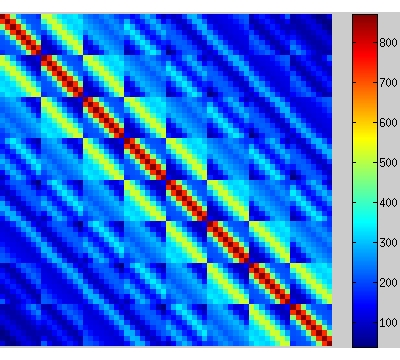
\includegraphics[width=\textwidth]{figures/ada}
    \caption{An example of $A^\dagger A$ for N=64 }
    \label{Figada}
  \end{center}
\end{figure}
